\documentclass[master=cws,english]{kulemt}
\usepackage[english]{babel}
\usepackage{graphicx}
\usepackage{subfig}
\usepackage{listings}
\usepackage{rotating}
\usepackage{threeparttable}
\lstset{breaklines=true}

\setup{title={Improving session security in web applications},
  author={Bram Bonn\'e},
  promotor={dr.\ L. Desmet \and Prof.\,dr.\ F. Piessens},
  assessor={Ir.\,P. Philippaerts \and G. Poulisse},
  assistant={\ P. De\ Ryck \and N. Nikiforakis}}
\setup{filingcard,
  translatedtitle={Verhoogde veiligheid van sessies in webapplicaties},
%
% UDC nummer is richtingafhankelijk. 
% Zie http://www.udcc.org/udcsummary/php/index.php
% voor het UDC nummer.
% Dit voorbeeld (519.6) verwijst naar 'Computational mathematics'
  udc=004.49,
  shortabstract={%TODO
    Hier komt een heel bondig abstract van hooguit 500
    woorden.
   }}
\setup{font=lm}


\usepackage[pdfusetitle,colorlinks,plainpages=false]{hyperref}
\usepackage[toc]{glossaries}
\makeglossaries

\begin{document}

\lstdefinelanguage{JavaScript} {
    morekeywords={
        break,const,continue,delete,do,while,export,for,in,function,
        if,else,import,in,instanceOf,label,let,new,return,switch,this,
        throw,try,catch,typeof,var,void,with,yield,
        },
    sensitive=false,
    morecomment=[l]{//},
    morecomment=[s]{/*}{*/},
    morestring=[b]",
    morestring=[d]',
    alsoletter={.}
}


\begin{preface}
I'd like to thank Lieven Desmet and Frank Piessens, my promotors, and Philippe De Ryck and Nick Nikiforakis, my supervisors, for suggestions and feedback. Lastly, thanks go out to all people who tested the extension.
\end{preface}

\tableofcontents*

\begin{abstract}
The \texttt{abstract} environment contains a more extensive overview of
the work. But it should be limited to one page.
\end{abstract}

\begin{abstract*}
Nederlandstalig abstract
\end{abstract*}

\listoffiguresandtables
%\renewcommand{\glossaryname}{List of Abbreviations}
\newglossaryentry{csrf}{name=CSRF,description={Cross-Site Request Forgery, an attack in which JavaScript is used to execute malicious code in the victim's browser}}
\newglossaryentry{css}{name=CSS,description={Cascading Style Sheets, used for defining the appearance of a web page}}
\newglossaryentry{dom}{name=DOM,description={Document Object Model, used by programming languages like JavaScript to access elements in an XML document or on a web page}}
\newglossaryentry{ip}{name=IP,description={Internet Protocol, the protocol used for routing datagrams over the internet. An IP address identifies a machine on the internet}}
\newglossaryentry{nat}{name=NAT,description={Network Address Translation, often used for allowing internet access to multiple machines via the same \gls{ip} address}}
\newglossaryentry{tld}{name=TLD,description={Top Level Domain, the last part of a \gls{url}, which determines the part of the domain that registered in the name space's root zone. Examples are \texttt{.com}, \texttt{.org} and \texttt{.co.uk}}}
\newglossaryentry{lcg}{name=LCG,description={Linear Congruential Generator, a generator for pseudorandom numbers based on recurrence}}
\newglossaryentry{sid}{name=SID,description={see `session ID'}}
\newglossaryentry{mac}{name=MAC,description={Message Authentication Code, a short piece of information providing data integrity and authenticity for a message}}
\newglossaryentry{mitm}{name=MitM,description={Man in the Middle, used to describe an attacker that is able to intercept traffic between the victim and some other principal}}
\newglossaryentry{psid}{name=PSID,description={Proxy Session Identifier, a second \gls{session id} which is attached and checked by a proxy to counter session fixation attacks}}
\newglossaryentry{session fixation}{name=session fixation,description={An attack in which the attacker tries to enforce a \gls{sid} upon the victim, so he is able to take over the session later on}}
\newglossaryentry{login session fixation}{name=login session fixation,description={A popular variation of the \gls{session fixation} attack, in which an attacker tricks the user into logging in with a predefined \gls{sid}}}
\newglossaryentry{session hijacking}{name=session hijacking,description={An attack in which the attacker tries to capture the victim's \gls{sid}, to be able to take over his session}}
\newglossaryentry{session id}{name=session ID,description={Session Identifier, a unique string of text used by the server to identify a user}}
\newglossaryentry{sop}{name=SOP,description={Same Origin Policy, the policy which states that \gls{dom} objects may only be accessed by principals having the same origin as the object}}
\newglossaryentry{ssl}{name=SSL,description={Secure Socket Layer (also known as TLS, or Transport Layer Security), used in \gls{https} to encrypt traffic between a client and a server}}
\newglossaryentry{http}{name=HTTP,description={HyperText Transfer Protocol, the protocol which is used by web browsers to communicate with web servers}}
\newglossaryentry{https}{name=HTTPS,description={HyperText Transfer Protocol Secure, a secure variant of \gls{http}, which uses encryption when transmitting data}}
\newglossaryentry{html}{name=HTML,description={HyperText Markup Language, the language used to structure web pages}}
\newglossaryentry{www}{name=WWW,description={World Wide Web}}
\newglossaryentry{web application framework}{name=web application framework,description={a framework providing the core functionality of web applications, which provides the foundation for web developers when building web applications}}
\newglossaryentry{cookie}{name=cookie,description={A piece of text made up of one or more name-value pairs stored by a website in the browser. Cookies are set by a website upon first visit, and subsequently included in every request made by the browser}}
\newglossaryentry{session cookie}{name=session cookie,description={A cookie containing a session identifier}}
\newglossaryentry{url}{name=URL,description={Uniform Resource Locator, a string that specifies the location of a resource}}
\newglossaryentry{xss}{name=XSS,description={Cross-Site Scripting, an attack wherein the attacker injects JavaScript into a legitimate page that will be executed by another user's browser when that user visits the page}}

\printglossaries

\mainmatter
\chapter{Introduction}

Over the last few years, the web has shifted from being a collection of pages containing static information to a dynamic and fully interactive platform. Where the Internet was once used only as an information repository, today it powers complex web applications, developed both to replace programs that were once running locally on a user's computer, and to provide whole new functionality that is possible only on the web. For this, web protocols to be used and extended in ways they were never imagined to be.

More than in the past, these web applications deal with sensitive personal information. Thanks to the emergence of web-based mail applications akin to Google's GMail and Microsoft's Hotmail, and social networks like Facebook and Netlog, a great deal of user information is stored on the servers of web applications. Moreover, shops have moved to the on-line world, and payments can be made on-line by using on-line banking or credit cards. Because many web applications handle such sensitive information, security of a user's information and identity is of utmost importance.

User authentication is handled in most web applications via the concept of web sessions. These allow users to use a web application without having to enter their login credentials for every action taken. Unfortunately, web sessions have many security weaknesses. OWASP, a leading organization in the field of web application security, rates `Broken Authentication and Session Management' as the third most important web application security risk \cite{Williams2010}.

In this thesis, the security of sessions in web applications is examined. The contributions of this thesis are threefold: firstly, we give a thorough overview of three important session attacks, together with a list of possible attack vectors for each of these attacks. Secondly, we compare different solutions that were proposed over the years to improve session security, and we inspect to what extent popular web frameworks provide protection against these attacks. Lastly, we propose a novel client-side approach to solving two important session attacks, which is the first one of its kind.

\chapter{About web sessions}

When a user visits a website, the web application often needs to remember which user it is interacting with. For this reason, the concept of a `web session' was invented. In this chapter we will see how web sessions work, and how their security can be improved.

\section{How web sessions work}\label{session-management}

To understand the need for web sessions, we first have to look at how web browsers communicate with web servers. The browser requests web pages by issuing \gls{http} requests to a web server \cite{Kurose2008}. The server subsequently responds to every request with an HTTP response containing the requested page. Unfortunately, HTTP is a stateless protocol, which means that the web server has no way of knowing whether two different requests come from the same user. Consider for example an online shop, where a user can fill its virtual shopping cart with different items available on the website. Without state, the web application would not be able to remember which items were associated with a user on subsequent page requests. Because of this, a mechanism is needed on top of HTTP to enable stateful communication between a web server and a client. This mechanism is known as a web session.

Web sessions work as follows:
\begin{enumerate}
	\item When the web server receives its first HTTP request from a particular client, it creates a \emph{session identifier} (also called a \gls{session id} or \gls{sid}) that it associates with this client. It then sends the newly generated SID to the client as part of the HTTP response.
	\item In subsequent communications, every request issued by the client to the server contains the received SID. Because the web server has associated this SID with a particular client, it will know who it is interacting with.
\end{enumerate}

\label{cookie-header}There are three ways in which session identifiers can be attached to requests and responses \cite{Jovanovic2006}. The first one, which is most common, makes use of \glspl{cookie} \cite{Kristol2001, Park2000}. Cookies are strings consisting of multiple name-value pairs which are set by the web server using the \texttt{Set-Cookie} HTTP header. Upon receiving a cookie, the browser stores it for a specified amount of time. It then attaches this cookie to every subsequent request made to the domain\footnote{The actual access control policy is a bit more complicated and will be discussed in section \ref{access-control}.} the cookie was set for. This is done by including the cookie as the value for HTTP's \texttt{Cookie} header. The process is graphically depicted in Figure \ref{fig:sessions-cookies}. It is clear that cookies are a very convenient mechanism for managing session identifiers. Because cookies can also be used for other purposes than session management, we will make a distinction between \emph{cookies} (which can be used for all sorts of state information) and \emph{\glspl{session cookie}} (which are cookies that store a SID) in this text.

\begin{figure}[ht]
	\centering
	\subfloat[via cookies]{
		\label{fig:sessions-cookies}
		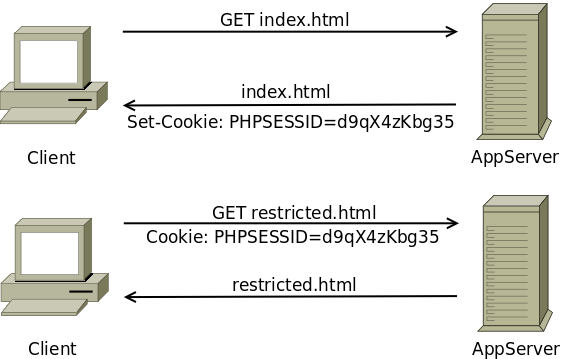
\includegraphics[width=.47\textwidth]{img/Sessions.png}
	}
	\subfloat[via URL rewriting]{
		\label{fig:url-rewriting}
		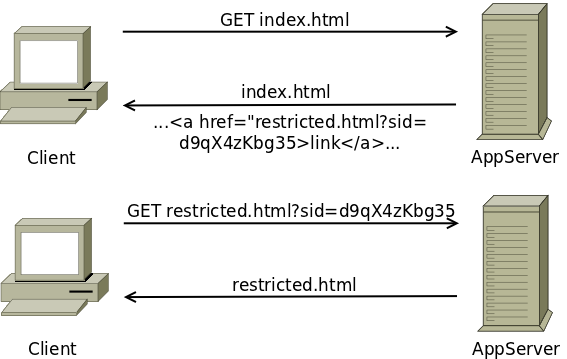
\includegraphics[width=0.47\textwidth]{img/url-rewriting.png}
	}
	\caption{Session management}
\end{figure}

The second possibility to include session information is via \emph{\gls{url} rewriting}. In this case, the web server appends the session ID as a parameter to every URL occurring in a response that points to a page on the same domain. Thus, when the user clicks a link on the served page, the request that is made contains the session ID as a parameter, and the server will know who made the request. This process is graphically depicted in Figure \ref{fig:url-rewriting}.

The third possibility is very similar to URL rewriting, but uses POST instead of GET parameters \cite{Johns2006}. Here, the session ID is included as a \texttt{<form>} element. When the user submits the form, the session ID is sent along with the request.

In this text, we will mostly focus on SIDs in cookies, because they are by far the most common. However, when appropriate, we will include information about session IDs in URLs.

There are two important things to note about session IDs. Firstly, there is no standardized way of doing session management. This means that different web applications will use different SID names, and that they will generate SID values in different ways. Secondly, SIDs are almost\footnote{We use the term `almost' because there is no standardized way of using SIDs. It can however safely be assumed that the majority of the pages encountered on the Web will use SIDs only to identify the user.} always used only as an enabler of server side storage, and not as the storage itself. This means that the SID only identifies the user, while all other state is saved at the server side. The server then associates the SID with the other state information stored for that particular session.

\section{Accessibility of session identifiers}

\label{access-control}\label{sop}The access policy for cookies states that a cookie is sent only to those pages that have the same (sub)domain as the page that set the cookie. Moreover, the page to which a cookie is sent must be on a path that is a suffix of the page that set the cookie \cite{Singh2010}. Cookies can also be accessed at the client side. For this, the \emph{Document Object Model} (or \emph{\gls{dom}}) is used. The Document Object Model provides a way for programming languages like JavaScript to access elements on a web page. It allows SIDs that are stored in a cookie to be accessed via the \texttt{document.cookie} property. For DOM objects, the \emph{Same Origin Policy} (or \emph{\gls{sop}}) is enforced \cite{Singh2010}. This policy states that web pages that want to access a certain DOM object (in this case, the cookie) must have the same origin as this object. The origin is defined as the tuple \texttt{<protocol,domain,port>}. Thus, the Same Origin Policy essentially allows only access to DOM objects which are on the same domain as (or on a subdomain of) the principal trying to access them. Moreover, it is required that the accessing principal uses the same protocol and port as the protocol and port where the DOM object originated from.

For SIDs that make use of URL rewriting, the situation at the server side is different. Here, the SID is only attached to requests that are the result of the user clicking a link on a web page, and only when the originating web page explicitly included the SID as a parameter in the link. At the client side, the session identifier is again available via the DOM, this time via the \texttt{href} attribute of the \texttt{<a>} element containing the URL. Thus, at the client side, the SOP again applies.

\section{Keeping web sessions secure}\label{secure-sessions}

It is important to ensure that a session identifier can only be known by the web server and the client that is identified by it. If an attacker is able to know a client's SID, he can use it to impersonate the client in the web application. One example is a webmail application\footnote{Examples of widely-used webmail applications are Google's GMail (\url{http://mail.google.com}) and Microsoft's Hotmail (\url{http://www.hotmail.com}).}, where an attacker could use the SID to be able to read and send e-mail on behalf of the client. Another example is the online shop, where an attacker could fill the client's virtual shopping cart with unwanted items. To prevent an attacker from knowing a client's SID, the SID should possess some properties. We describe these properties in this section.

\subsection{Unguessable by an attacker}

An attacker should not be able to guess the value of a user's session ID. For this, the following properties are necessary:

\subsubsection{Randomness}
To be unguessable, a session identifier should appear like it could be any random string of text. Random in this case means that session identifiers should have \cite{Nikiforakis2010, Farrell2011, rfc4086}:
\begin{description}
	\item[high entropy] The higher the number of bits that are necessary to represent a string, the higher the string's entropy is.
	\item[low correlation] If SIDs are correlated, an attacker is able to derive (part of) SIDs that will be generated from SIDs which were already generated. As a consequence, an attacker would be able to predict a victim's session ID from his own session ID.
	\item[a high number of possible values] This is related to both high entropy, and to sufficient length (which will be discussed shortly hereafter).
\end{description}
It must also be noted that it is not sufficient for session IDs to be only statistically random: they have to be cryptographically random \cite{Fu2001}. This means that more than just an \gls{lcg} %TODO: Citation naar cursus Modellering&Simulatie!
is needed to generate the SIDs.

\subsubsection{Sufficient length}
To prevent successful brute forcing attacks, wherein an attacker exhaustively tries lots of possible values, a session ID should be of sufficient length. The expected number of seconds required to guess any one valid session identifier is given by the equation \cite{OWASP2009a}:
\[
	\frac{2^B + 1}{2A \cdot S}
\]
where $B$ is the number of bits of entropy in the SID, $A$ is the number of guesses an attacker can try each second, and $S$ is the number of valid SIDs at any given time.

OWASP, a leading organization in the field of web application security\footnote{More information about the OWASP project can be found at \url{https://www.owasp.org/}.}, recommends a session ID length of at least 128 bits \cite{OWASP2009a}.

\subsection{Unavailable to an attacker}
If an attacker is able to read the value of the victim's SID, the victim's session is compromised. Because of this, it is of utmost importance that the SID value is never visible to anyone but the legitimate user and the web servers on the domain the SID was set for. In this section, we only describe some default properties to achieve this. We will go into more detail about making cookies unavailable to an attacker in section \ref{general-security}.

\label{secure-flag}SIDs that are set via cookies are, by default, transmitted as clear text. This means that, in an insecure channel like the Internet, an eavesdropper is able to intercept the cookie value. An eavesdropping attacker can thus take over a user's session. Cookies can also be sent over a secure (TLS, but most often referred to as \gls{ssl}) connection \cite{rfc4346}. In this case, the requests and responses (and thus, the cookie value) are encrypted, and the attacker is unable to extract the cookie wen viewing one of these messages. Care must be taken, then, that the cookie value is never sent in the clear; otherwise its value can still be compromised. To ensure that this is the case, the \texttt{secure} flag should be enabled when setting a cookie \cite{Fu2001, rfc2965}. This flag demands that the browser may never send the cookie over an unencrypted connection.

When an SID which is set via a cookie will never need to be accessed via JavaScript, it is best to enable the \texttt{HttpOnly} flag when setting the cookie \cite{Nikiforakis2010}. When this flag is enabled, the browser will only allow the cookie to be accessed via \gls{http}. Accessing a cookie set using the \texttt{HttpOnly} flag via JavaScript will be disallowed. With URL rewriting, it is not possible to state that the SID may not be available to client-side JavaScript. Indeed, a link containing the SID will always be available as a DOM object.

\subsection{Short lifetime}\label{lifetime}
A third way of making sessions more secure is to ensure that they have a limited lifetime \cite{Fu2001}. This has two advantages:
\begin{itemize}
	\item The shorter the lifetime of a SID, the less time an attacker has to brute force it.
	\item In case the attacker was able to capture the SID, the lifetime of the SID determines how long the attacker is able to use it for impersonating the victim.
\end{itemize}

Additionally, limiting the lifetime of a session identifier makes sure that a user will be logged out eventually. This is convenient in case a user forgets to log out when he stops using the web application \cite{OWASP2009a}. %TODO: better citation needed

\subsubsection{Limiting the SID's lifetime}\label{limiting-lifetime}
The lifetime of a cookie can be limited by using the \texttt{expires} attribute when setting the cookie. However, care must be taken that the session is also invalidated at the server side, because the attacker could otherwise still use the cookie after it expired at the victim's browser \cite{Kolsek2002}.

Another way of limiting the lifetime of a session identifier is presented by K. Fu et al. \cite{Fu2001}. By including a timestamp as part of the SID value, a server can determine whether the SID is still valid without having to save the SID's expiration time as part of its state. It is important to note that, because the timestamp is appended to the normal session identifier, this requires the complete SID value (including the timestamp) to be signed by the server. Otherwise, an attacker could just change the timestamp part of the SID to extend its lifetime. The signing can be easily achieved by letting the server create a \gls{mac} of the entire SID, and appending this MAC to the SID value. A disadvantage of this approach is that there is no possibility of revoking SIDs without keeping extra server state.

\subsubsection{Renewing the SID}\label{renewing-sid}
Fortunately, the user does not have to re-authenticate every time he gets a new session ID. Only three steps have to be performed by the server to provide a client with a new SID:
\begin{enumerate}
	\item Generate a new session ID.
	\item Associate the new SID with the existing user. For this, any server side state which was attached to the old SID should be attached to the new SID instead \cite{Wasser2007}.
	\item Make sure the client uses the new SID instead of the old one. This can be done by attaching a \texttt{Set-Cookie} header to the next HTTP response, containing the new SID value. The browser will notice that the cookie name is the same as the old SID, and will therefore update the old value. Alternatively, when URL rewriting is used, the web server has to make sure that all links on subsequent web pages served to this client include the new SID value.
	\item Invalidate the old session identifier.
\end{enumerate}

\subsection{Using a session management framework}

Problems occur in lots of web applications because they implement their own session management. As we will see in section \ref{frameworks}, lots of web frameworks have thoroughly tested session management already built-in. Because it is very easy to make mistakes when providing security, it is recommended to make use of an existing session management framework. Using such a framework does not completely relieve the web developer of all tasks associated with session management: he must still make sure that the framework is configured correctly, and that other channels (for example, JavaScript) don't pose any security issues.

\chapter{Session attacks}\label{attacks}

Now that we know how web sessions work, we look into ways in which attackers are able to abuse them. In this chapter, we will see how an attacker can use the concept of web sessions to impersonate a legitimate user on a website.

\section{Background: cross-site scripting}\label{xss}

Cross-site scripting (or \gls{xss}) is not a session attack in itself. Instead, it is the exploitation of a vulnerability in some websites which can be of great use when executing one of the other attacks described below.

In a cross-site scripting attack, the attacker exploits a vulnerability in a website to inject his own JavaScript code into this page \cite{DiLucca2005}. The code will then be executed in the browser of any user that loads the page with the injected code.

\subsection{Variants of cross-site scripting}
There are two forms of cross-site scripting: persistent and non-persistent XSS. In this subsection, we describe their differences and give some examples of possible attack scenarios for each of them.

\subsubsection{Persistent (stored) XSS}
In a persistent attack, the attacker makes the web application store the script code in a database. The complete scenario goes as follows:

\begin{enumerate}
	\item The attacker provides his malicious code as input to the web application.  The web server stores this input (and thus the script code) in the database to be able to provide it to clients later on.
	\item The victim requests a page containing content generated by the attacker. The server returns the page containing the attacker's JavaScript.
	\item The victim's browser thinks that the script code is part of the requested web page and executes it.
\end{enumerate}

This attack variant is graphically illustrated in figure \ref{fig:persistent-xss}.

\begin{figure}[ht]
	\centering
	\subfloat[persistent]{
		\label{fig:persistent-xss}
		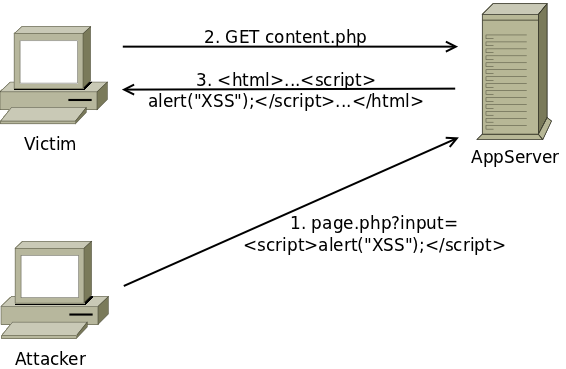
\includegraphics[width=.45\textwidth]{img/persistent-xss.png}
	}
	\subfloat[non-persistent]{
		\label{fig:nonpersistent-xss}
		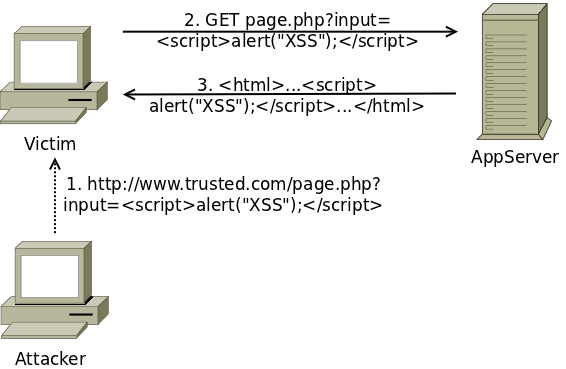
\includegraphics[width=0.45\textwidth]{img/nonpersistent-xss.png}
	}
	\caption{The cross-site scripting attack}
\end{figure}

An example of a web application that will store user input in a database to serve it later it is a bulletin board (phpBB\footnote{\url{http://www.phpbb.com/}} is a well-known example), where a user can create forum posts that will be read by other users of the bulletin board. When an attacker inserts script code into a post, the code will be executed at the browser of every user reading that post.

A more recent example is found in social networking sites like Facebook\footnote{\url{http://www.facebook.com}}. Here, a user can place information on his own page, or the pages of other people. This information will then be served to the user's friends.
% Image

\subsubsection{Non-persistent (reflected) XSS}
In a non-persistent attack, the script code is never stored at the server side. Instead, code that was part of a request is immediately reflected back to a client's browser as part of the response page. The steps are as follows:

\begin{enumerate}
	\item The attacker tricks the victim into opening a malicious link containing script code.
	\item The victim opens the link, and unknowingly makes a request containing script code to the server.
	\item The server reflects this script code back to the victim as part of the response.
	\item The victim's browser thinks that the script code is part of the requested web page and executes it.
\end{enumerate}

This attack variant is graphically illustrated in figure \ref{fig:nonpersistent-xss}.

An example of this is a search form, where a website returns the term the user searched for, without stripping any script data that might be inside. If doing a search by going to the URL \url{http://www.trusted.com/search?q=searchterm} makes the website return ``x results for \emph{searchterm}'', the attacker can replace \emph{searchterm} by script code that will execute at the client that loads the search results. The attacker can then trick a user into clicking the link, causing the JavaScript code to be executed in his browser.

Another example of a scenario where a website might return data found in the URL is the `Page not found' error page \cite{Kirda2006}. Here, the name of the page that could not be found is often included as part of the error message. Thus, an attacker can craft a link wherein he requests a page with name \texttt{<script>alert("XSS succeeded");</script>} to make a client's browser execute JavaScript code.
% Image

\subsection{Including the script code}\label{injecting-script}
There are multiple ways in which script code can be included in a web page. Since all of these can be leveraged by an attacker to inject his code into a web page, it is important that web developers are aware of all of them. T. Jim et al. give a good overview of different approaches to including JavaScript code \cite{Jim2007}, of which we will describe the most important ones here:
\begin{description}
	\item[between \texttt{<script>} tags] This is the most obvious way of including JavaScript in a web page. All code between these tags will be executed as soon as the browser encounters it.
	\item[using the \texttt{<script>} tag's \texttt{source} parameter] This parameter can be set to point to an external piece of JavaScript. As such, an attacker is able to make a website load JavaScript code from another domain. An advantage for the attacker is that the actual injected string is shorter, bypassing message length limits.
	\item[as the URL of the background image] An attacker can insert a tag similar to \texttt{<div style="background-image: url(javascript:alert('XSS');" />} or \texttt{<style>.bar\{background-image:url("javascript:alert('XSS');");\}</style>} (where \texttt{bar} is the class of an object in the page) to make the browser execute JavaScript, thinking it is loading the background image.
	\item[using the \texttt{onload} parameter of the \texttt{<body>} tag] This tag is used for code that should be executed once the browser has completed loading the page.
\end{description}

It must also be noted that attackers can use different possible encodings to inject JavaScript, so as to circumvent server-side JavaScript checkers, while still being able to execute at the client side \cite{Jim2007}. For example, the encoding of (parts of) a web page can be changed using the \texttt{encoding} and \texttt{charset} attributes of various HTML tags \cite{Ishida2010}. Some browsers also allow strings to contain JavaScript that is split over multiple lines \cite{Jim2007}. Lastly, JavaScript can be split over multiple  \texttt{<![CDATA[\dots]]>} tags, making it much harder to detect.

\subsection{The danger of cross-site scripting}\label{xss-problem}

One danger of persistent XSS is immediately clear: websites that do not belong to an attacker can still be used by the attacker to execute malicious code at a user's browser. The user, thinking that a known site will only execute trusted code, can fall victim to the attacker without expecting it.

There is, however, a bigger problem which applies to both persistent and non-persistent XSS: the problem of trust. Normally, the attacker's code would be subject to the \gls{sop} (described in section \ref{sop}), making him unable to access elements of a domain that he does not own. However, when the attacker's code is able to execute from within a trusted domain (as is the case in an XSS attack), this code may access the elements belonging to the trusted domain \cite{Klein2002}. This gives the attacker the ability to read information from, and write information to, elements in the trusted domain.

The situation is even worse when the attacker's code is loaded from a different domain (because the attacker injected the script code by using the \texttt{<script>} tag's \texttt{src} attribute, for example). When this is the case, the script code is also allowed to communicate with the domain it was loaded from \cite{Singh2010}, i.e. the attacker's domain. Because of this, the attacker is able to capture information from a trusted domain and subsequently send this information to his own domain. This will be a major attack vector for the session hijacking and session fixation attacks, as we will see in the next sections.

\section{Session hijacking}\label{hijacking}

In the session hijacking attack, an attacker tries to take over a victim's session by capturing his \gls{session id}. Using this SID, the attacker can make the server think that he is the victim. First, we describe the attack scenario. Afterwards, we will see how the attacker can capture the victim's session ID.

\subsection{Attack scenario}

The session hijacking attack works as follows \cite{Nikiforakis2010}:

\begin{enumerate}
	\item The victim establishes a new session at the server. This is done automatically by the victim's browser either when he first visits the page or when he logs in (depending on the web application).
	\item The attacker captures the session ID that corresponds to the victim's created session by using one of the methods described in section \ref{capturing}.
	\item The attacker makes a request to the server, attaching the captured session ID as his own. Because the server has no other means of distinguishing between the victim and the attacker, it thinks that it is the victim that made the request. Thus, the attacker is now able to impersonate the victim at the server.
\end{enumerate}

These steps are graphically illustrated in figure \ref{fig:hijacking}.

\begin{figure}[ht]
	\centering
	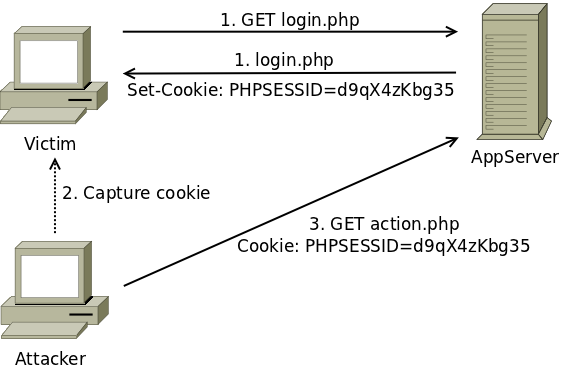
\includegraphics[width=0.50\textwidth]{img/hijacking.png}
	\caption{The session hijacking attack}
	\label{fig:hijacking}
\end{figure}

\subsection{Capturing the session ID}\label{capturing}

There are lots of possible ways in which an attacker can capture a victim's session ID. We list the most important ones here.

\subsubsection{Via a (passive) man-in-the-middle attack}

In a man-in-the-middle (or \gls{mitm}) attack, an attacker is able to read traffic that passes between the client and the server. This is usually the case because both the client and the attacker are using the same network unencrypted WiFi network, or because they share the same network hub.

The session identifier is, by default, sent over the network as an unencrypted string of text, both when using cookies as when making use of URL rewriting. Because of this, an attacker able to read all network traffic can easily extract the SID from the \texttt{Cookie} header in one of the user's requests, or even from the \texttt{Set-Cookie} header in the server response setting the cookie \cite{Adida2008}.

This problem has been known for some time, and has recently again received some attention thanks to tools like Hamster \cite{Graham2007} and Firesheep \cite{Butler2010}, which make a session hijacking attack almost trivial when the victim is on an insecure network.

\subsubsection{Via cross-site scripting}

The \gls{xss} attack described in section \ref{xss} can also be used to steal a victim's session ID. For this, the attacker uses the \texttt{<script>} tag's \texttt{src} attribute to load script code from his own domain into a web page on the domain he wants to acquire the cookie from. Because the script code is loaded from within a page on the target domain, the attacker has access to both the target domain's cookie via the \texttt{cookie} attribute of the \texttt{domain} \gls{dom} object (for SIDs set in cookies), and to all links on the current page (for SIDs used via URL rewriting). However, since the script code was loaded from the attacker's domain, it is also allowed to communicate to that domain (see section \ref{xss-problem} and \cite{Klein2002} for more information). Because of this, the attacker is able to forward the target domain's cookie to his own domain, effectively capturing the client's SID.

\subsubsection{Via the referer header}

A third possible SID leak occurs when the browser attaches the \texttt{referer} header to a request going to another domain \cite{Fu2001}. The \texttt{referer} header is used to transmit the resource from which the request-URL was obtained \cite{rfc2616}. If SIDs are included in the URL (as is the case with URL rewriting), the website receiving the \texttt{referer} header as part of the request can extract the client's SID for the web application that contained the link.

If, for example, a social networking website manages sessions via URL rewriting, an attacker could share a link to his own website on this website. When another user clicks the link, a request is made to the attacker's web server. This request contains the URL of the current page, and thus the user's SID for the social networking website, in the \texttt{referer} header, making it available to the attacker.

Sometimes, the \texttt{referer} header is suppressed in the network or by the browser, especially for cross-domain requests \cite{Barth2008}. Unfortunately, the percentage of requests where the \texttt{referer} header is stripped is still small enough to consider leaking of SIDs via this channel a significant threat.

\subsubsection{Via the user}

Lastly, it is also possible that the user unknowingly leaks his own session identifier. This is the case when the user shares a link to a page for a website that uses URL rewriting \cite{Johnston2004}, for example via email or a social networking site. When another user clicks the shared link, he will automatically take over the first user's session. Thus, the second user essentially performs a session hijacking attack on the first user, possibly without even realizing it.

This problem, together with the possibility of leaking SIDs via the \texttt{referer} header, provides a strong argument against using URL rewriting for session management.

\section{Session fixation}\label{fixation}

In the session fixation attack, as in the \gls{session hijacking} attack (section \ref{hijacking}), an attacker's goal is to be using the same session as a victim. However, instead of capturing the victim's \gls{session id}, the attacker forces the victim to use a SID that is known in advance. We will first describe the steps necessary to execute this attack. Afterwards, we list the ways in which the attacker can force a victim to use a certain session ID.

\subsection{Attack scenario}

The session fixation attack works as follows \cite{Kolsek2002}:

\begin{enumerate}
	\item The \emph{attacker} establishes a new session at the server. He does this by sending a request that doesn't include a SID. The server will then attach a newly generated
SID to the response. Some servers also accept random SIDs\footnote{By random SIDs, we mean that these SIDs don't need to be generated by the server in advance. A random SID can be sent by the client on his first request.} \cite{Shiflett2004}. If this is the case, the attacker can just make up a new SID, and no request needs to be made.
	\item The attacker forces the victim to use the newly created session ID. We will see how this can be done in section \ref{injecting-sid}.
	\item The victim uses his credentials to log in at the server. The SID that was injected at the client's web browser will automatically be attached to the request. Because of this, there now exists a session at the server in which the victim is logged in. That session is identified by a SID which is known by the attacker.
	\item The attacker makes a request to the server, attaching the captured session ID as his own. This makes the server think that it is the victim that made the request. Thus, the attacker is now able to impersonate the victim at the server.
\end{enumerate}

These steps are graphically illustrated in figure \ref{fig:fixation}.

\begin{figure}[ht]
	\centering
	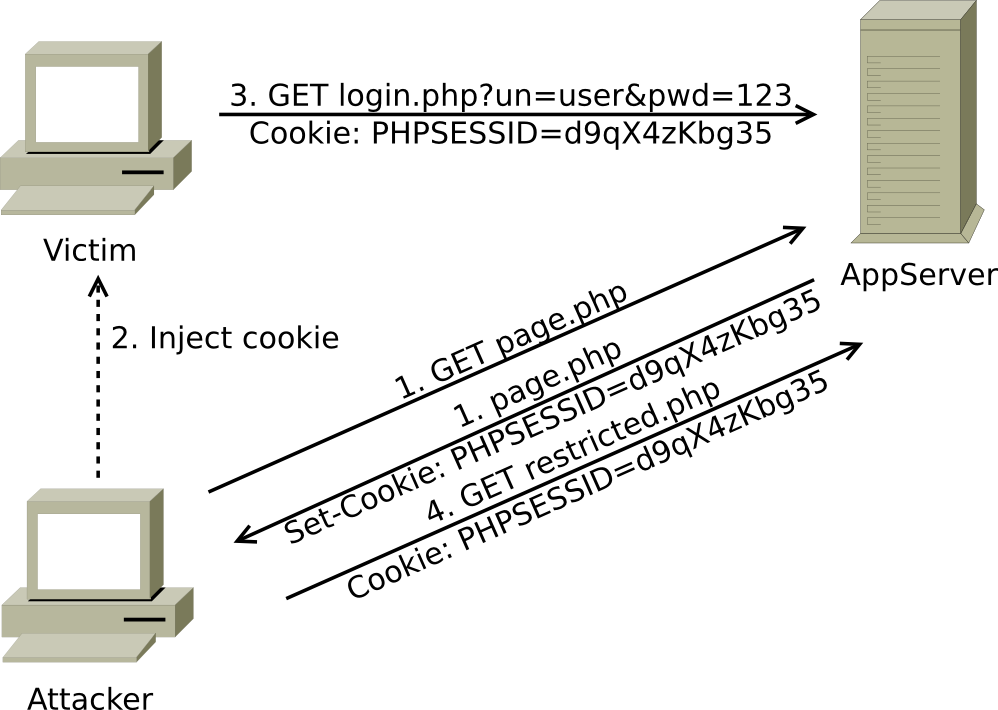
\includegraphics[width=0.50\textwidth]{img/fixation.png}
	\caption{The session fixation attack}
	\label{fig:fixation}
\end{figure}

\subsection{Injecting a session ID}\label{injecting-sid}

In this section, we describe the most important attack vectors the attacker can use to inject a session ID into the victim's browser.

\subsubsection{Via GET or POST parameters}

If the target website accepts session ID's in \glspl{url} (see section \ref{session-management}), the attacker can craft a link of the form \url{http://www.target.com/login.php?PHPSESSID=d9qX4zKbg35}, where he chooses the desired session ID \cite{Johns2011}. He then sends this link to the victim, or places on the target website as part of a \gls{xss} attack. When the victim clicks the link, the request sent to the target server will contain the attacker's SID in the URL, causing the web application to think it is the victim's session ID. Alternatively, the attacker can force the victim to visit the URL by using a HTTP redirect \cite{rfc2616} to make the victim's browser automatically load the page \cite{Shiflett2004}. However, this requires the attacker to be able to perform a XSS attack, or the victim to visit the attacker's page.

In case the target website uses POST instead of GET parameters for session management, the link can be replaced by an automatically submitting form \cite{Kolsek2002,Bontrager2005}.

Note that, for a website to accept session IDs via GET or POST parameters, it doesn't have to do its session management via URL rewriting by default. Indeed, multiple frameworks provide URL rewriting as a fallback for browsers that don't support cookies, causing them to be vulnerable to session fixation via URL rewriting \cite{Condit2006,Holovaty2008}.

\subsubsection{Via cross-site scripting}

If an attacker is able to inject script code into the target site (using one of the methods described in section \ref{injecting-script}), he can use this script code to set or replace the \gls{session cookie} with the desired value. This is done by editing the \texttt{document}'s \texttt{cookie} property \cite{Kolsek2002} or by using the \texttt{cookie.write()} function \cite{Johns2011}.

Alternatively, the attacker can use the HTML \texttt{<meta>} tag to set the cookie. For this, he injects the following line of HTML code into the target web page:
\begin{lstlisting}
<meta http-equiv=Set-Cookie content="PHPSESSID=d9qX4zKbg35">
\end{lstlisting}
where the name and value of the session cookie are chosen by the attacker \cite{Kolsek2002}.

\subsubsection{Via subdomain cookie setting}

Sometimes, an attacker is able to take over a subdomain of the target website because it is more vulnerable than the parent domain, or because he has legitimate access on the subdomain. Normally, setting a cookie on a subdomain would not have any effect on the parent domain. Indeed, as we described in section \ref{access-control}, cookies will only be used for the same domain as the one that set them, or for one of its subdomains. Thus, a cookie set on a subdomain will not be used for its parent domain. Because of this, it would seem that session fixation is not possible from within a subdomain.

There is, however, a possibility to set a cookie for a parent domain by using the cookie's \texttt{domain} parameter when setting a cookie \cite{rfc2109}. To do this, consider the case where the attacker was able to take over the domain \url{vulnerable.target.com}. He can then use this domain to set a cookie for \url{target.com}, and all of its subdomains, by specifying the cookie as \texttt{PHPSESSID=d9qX4zKbg35;domain=.target.com} (notice the `\texttt{.}' preceding \texttt{target.com}). This effectively allows an attacker that has access to a subdomain to execute a session fixation attack on a parent domain \cite{Kolsek2002}.

\subsubsection{Via HTTP response splitting / header injection}

There is another attack that can be used by an attacker to inject a cookie on the victim's machine. In a HTTP response splitting attack, the attacker tricks the victim's browser (or an in-between proxy) into thinking that two HTTP responses were sent by the target server, whereas both are actually part of the same HTTP response \cite{Klein2004}. The interesting part for the attacker is that the contents of one of the two responses can be chosen by himself. Because of this, an attacker is able to insert a \texttt{Set-Cookie} header containing the desired session identifier, effectively injecting the SID into the client's browser \cite{Johns2011}.

\subsection{Other dangers of session fixation}

It seems that the only benefit an attacker has from performing a session fixation is that he can take over the temporary session of another user. There is, however, another issue: an attacker is also able to force a victim to be logged in under the attacker's account. He can do this by logging in first, and subsequently forcing the victim to use the attacker's session ID. This has two major implications \cite{Barth2008}:
\begin{itemize}
	\item An attacker can track the victim's actions on the target web application by making use of logging functionality offered by this application. For example, most major search engines offer the option to log the user's search history\footnote{Google, for example, offers an overview for all terms you searched for at \url{http://www.google.com/searchhistory/}.}, allowing an attacker who is able to perform a session fixation attack to access this highly sensitive information.
	\item On domains that allow the embedding of trusted scripts, it creates the ability for an attacker to execute \gls{xss} attacks. Until recently, iGoogle\footnote{\url{http://www.google.com/ig}} offered the ability to embed trusted scripts on your own personal homepage \cite{Barth2008}. Because of this, an attacker who is able to perform a session fixation attack has the ability to offer scripts to a victim from within the \texttt{google.com} domain. He does this by adding a script to his own homepage, and subsequently imposing his own SID upon the victim's browser. Thus, the next time the victim visits iGoogle, the attacker's home page will be loaded, and the script will be executed.
\end{itemize}

As we can see, the session fixation attack is more venomous than would be expected when first looked upon. Because of this, we developed a client-side solution to session fixation, which will be described in chapter \ref{fixation-solution}.

\section{Cross Site Request Forgery}\label{csrf}

The cross site request forgery (also called \gls{csrf} or session riding) attack is different from the \gls{session hijacking} and \gls{session fixation} attacks in the sense that the attacker will not try to completely take over a victim's session. Instead, it leverages the victim's browser's implicit authentication to make requests in the name of the client. The attacker accomplishes this by compelling the victim's browser into issuing the request. This can be useful, for example, when the victim is logged in at the website of his bank. In this case, the attacker can use the victim's implicit authentication to transfer money from the victim's account to his own account.
Before we see the ways in which the attacker can make a victim's browser issue requests, let us first look at the complete attack scenario.

\subsection{Attack scenario}

The CSRF attack is made up out of the following steps:

\begin{enumerate}
	\item The attacker forces the victim's browser to send a request to the server (we will see how in section \ref{forcing-request}). It is the attacker that chooses the contents of this request.
	\item The browser, thinking that it is a legitimate request made by the victim, automatically attaches the victim's authentication information.
	\item The browser sends the request to the target server. This server uses the request's authentication information to determine that the request was made by the victim. Thus, the server executes any action that was requested by the attacker as if the victim requested it.
\end{enumerate}

The different steps of the CSRF attack are graphically illustrated in figure \ref{fig:csrf}.

\begin{figure}[ht]
	\centering
	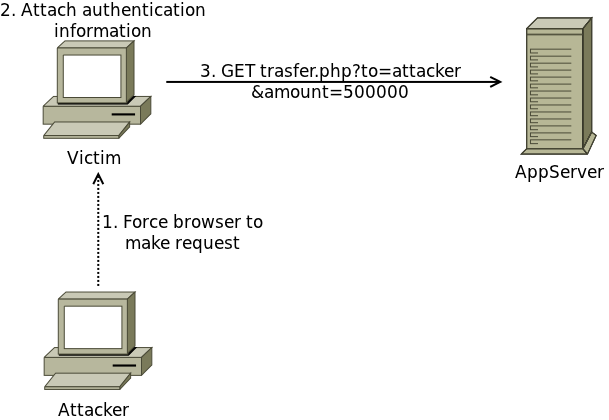
\includegraphics[width=0.50\textwidth]{img/csrf.png}
	\caption{The cross site request forgery attack}
	\label{fig:csrf}
\end{figure}

\subsection{Forcing the browser to make a request}\label{forcing-request}

\chapter{Session attack countermeasures}

In this chapter, we discuss some general countermeasures to the session hijacking and session fixation attacks. We also briefly describe some solutions to cross site scripting attacks, because of their importance in session attacks. The discussion of more specific countermeasures is deferred to section \ref{related-work}, where we talk about countermeasures related to our own solution. % TODO: check of dit nog overeenkomt met uiteindelijke lay-out

\section{Server-side countermeasures}

This section is dedicated to server-side countermeasures against session hijacking and session fixation. We first describe some general security measures that a web developer can take to secure his web application. Afterwards, we inspect different web frameworks to see how they safeguard against the aforementioned session attacks.

\subsection{General security measures}\label{general-security}

Different security measures may be taken by web application and web framework developers to secure their web applications. In this section, we discuss to what extent these measures provide security against session hijacking and session fixation attacks.

\subsubsection{Renewing the session identifier}\label{renewing}

The practice of renewing the session identifier (see section \ref{renewing-sid}) can provide excellent protection against \gls{login session fixation} attacks. Indeed, if the web application renews the session identifier every time the authentication status of a user changes, the SID which was enforced by the attacker won't be valid anymore once the victim has logged in. As an example, this can be accomplished in PHP by using the following code snippet \cite{PHPregenerate,Johns2011}:

\begin{lstlisting}[language=PHP]
if ($authentication_successful) {
    $_session["authenticated"] = true;
    session_regenerate_id();
}
\end{lstlisting}

To make sure that the session identifier is changed on every authentication change, it can be made to contain specific user information (like the username). In this case, when the authentication state changes, the session identifier has to change, too. If this is used in combination with a server \gls{mac} (as described by Fu et al. \cite{Fu2001}), an attacker is not able to include another username in the value himself.

Renewing the session identifier regularly is also benefical for preventing session hijacking attacks. As was discussed in section \ref{lifetime}, the shorter the lifetime of a session identifier, the more difficult it will be to capture, and the less useful it will be if it has been captured \cite{Fu2001}.

Keeping in mind the previous discussion, one might assume that it is best to renew a session identifier as often as possible. Consider, however, the case where the session identifier is renewed on each request. In this case, every request would result in a new session cookie being set at the user's browser, with the old session cookie being invalidated. When issuing concurrent requests, the web application would only acknowledge the first request that arrived at the server. The second request would contain the (by then) invalidated session identifier, causing it to be rejected. Because of this, the browser would be allowed to issue only one request at the same time. Similarly, this would pose a problem when browser plugins communicate with the server, as well as with asynchronous requests.

\subsubsection{Using HttpOnly cookies}\label{httponly}

When setting a cookie in the user's browser, a web server can use the cookie's \texttt{HttpOnly} flag to indicate that the browser should only allow access to this cookie via \gls{http}. As a consequence, script code will not be able to access or edit the value for such cookie, and \gls{xss} attacks can be prevented \cite{HttpOnly}.

Singh et al. have shown that it is sometimes still possible for an attacker to read or manipulate a HttpOnly cookie via JavaScript \cite{Singh2010}. Fortunately, our experiments show that the issue of Firefox allowing cookie writes to HttpOnly cookies has since been solved. However, as we will describe in section \ref{httponlyremark}, we have discovered yet other techniques which allow an attacker to circumvent these browser policies. As such, we must conclude that, while marking a cookie as HttpOnly does prevent an attacker from accessing the cookie via JavaScript, it does not prevent him from using XSS to inject a chosen value for this cookie into the victim's browser.

\subsubsection{Secure connections}\label{ssl}

Secure connections can be used to make sure that a session identifier can not be intercepted by a passive \gls{mitm} attacker. In this case, as already noted in \ref{secure-flag}, care must be taken that cookies can never be sent over an unsecure connection. This can be done by setting the \texttt{secure} flag for cookies that will be used only over a \gls{ssl} connection.

Recently, some work has been done to make deployment of HTTPS more widespread \cite{Hodges2010,Jackson2008}. Unfortunately, there are still some drawbacks to using HTTPS for every page \cite{Adida2008}. At the server side, HTTPS is very costly: every connection needs computationally intensive SSL operations to be performed. At the client side, browser caching works differently under SSL, and websites have to be completely transmitted before they can be rendered (because the validity is checked for the entire page).

\subsubsection{Checking other request headers}

Similar to the \texttt{Cookie} header we discussed in section \ref{cookie-header}, a \gls{http} request can contain many other headers \cite{rfc2616}. Some of these headers provide information that can be used to identify a user. For example, the \texttt{User-Agent} header contains information about a user's browser and operating system, while the \texttt{Accept-Language} header lists the languages the user is willing to receive.

A web server can gain some extra certainty about whether it is interacting with the user corresponding to the session ID in the request by comparing some of the header values to those in the last request with the same session ID. Indeed, because an attacker is probably using a configuration which is different from the victim's, the attacker's requests will have different header values. Thus, when certain header values differ between requests, it is possible that a session hijacking or session fixation attack occurred.

The question is then: which headers could be considered to give enough user-specific information, without changing over time? The \texttt{User-Agent} header is obviously the best candidate. Unfortunately, web proxies are known to modify this header \cite{ShiflettHijacking}. Another header which could be considered is the \texttt{Accept} header, which lists the types of content the user's browser will accept. The problem with this header is that in Internet Explorer, its value can change over time \cite{ShiflettHijacking}. The \texttt{Accept-Language} header could be considered. However, different browsers might have the same default value (\texttt{en-US}) for this header. The same goes for the \texttt{Connection} and \texttt{Cache-Control} headers. Other headers are too susceptible to change, and shouldn't be used.

Another problem with using HTTP headers for this purpose is that they are easily guessed by an attacker. Indeed, for most headers, only few options are possible, with even less options being very probable. Furthermore, even in the case that an attacker would not be able to guess the header values, he only needs to read a single request (to whatever server) from the victim to know what header values to use. He can get a request from the victim by intercepting it, or by tricking the victim into visiting his own website.

Thus, while checking the headers might raise the barrier for attackers, it is by no means a complete solution against any of the described session attacks.

\subsubsection{Checking the IP address}

Similar to request headers, the \gls{ip} address can be used by the web server to ensure it is interacting with the same user as before. Unfortunately, this approach also suffers from some problems. Firstly, IP addresses can be captured in much the same way as HTTP headers. An attacker can then easily change the source IP address for his own packets to impersonate the victim. Secondly, when both the victim and the attacker are behind the same \gls{nat} proxy (as is often the case in session hijacking attacks over a wireless network), they are using the same IP address \cite{Johns2011}. In this case, the server can not distinguish the attacker and the victim based on IP address. Lastly, requiring that the IP address stays the same over time can also cause some problems to the legitimate user: with users changing the location of their notebook or cell phone, the IP addresses of these devices will change when roaming, causing them to be denied access to a web application that checks their IP address. Moreover, some networks only issue dynamic IP addresses to their users. Because of these reasons, it can not be assumed that a user is uniquely tied to a single IP address.

As was the case for checking other request headers, checking the IP address can not be considered a complete solution to any session attack.

\subsubsection{Cookies vs. URL rewriting and form elements}\label{url-vs-cookies}

As we described in section \ref{session-management}, there are three major methods for doing session management: via cookies, via URL rewriting and via form elements. We compare the advantages and disadvantages of these methods here.

A first major disadvantage of URL rewriting was already discussed in section \ref{leaking-via-user}: the session identifier can leak when a link is shared with someone else (for example, via e-mail or a social networking site) \cite{Johnston2004}. A leak can also occur when the \texttt{referer} HTTP header is included in a request to another website: since the URL in the referer header contains the user's session identifier, this identifier is visible to the other website \cite{Fu2001}.

A disadvantage which is shared by both the `URL rewriting' and `form elements' methods is that the injection of a session identifier (with the objective of executing a session fixation attack) requires little effort from an attacker. Indeed, as we saw in section \ref{get-or-post}, such an injection attack is reasonably straightforward.

There is, however, also an advantage of choosing URL rewriting or form elements over cookies, in particular when looking at the cross site request forgery attack. Recall that, to execute a \gls{csrf} attack, an attacker tricks the victim's browser into issuing a request. For this, he  has to create a URL or a form containing the right GET/POST parameters for the attack. However, if the SID is one of the parameters that must be included in the request, the attacker does not know all required parameters, and is therefore not able to create a complete request \cite{Johnston2004}.

It is clear that choosing which method to use for managing sessions requires careful weighing of the advantages and disadvantages of each method. It could be argued that cookies provide more security since they make leaking of session identifiers less likely. Indeed, it is often recommended to use cookies instead of URL rewriting for session management \cite{Zhong2006,Vamosi2006}. An even better option is to use a combination of cookies and POST or GET parameters. As we will see in section \ref{xss-countermeasures}, this is what many CSRF countermeasures try to do \cite{Jovanovic2006,Johns2006}. In addition, some (mobile) web browsers don't support cookies, requiring the use of POST or GET parameters when session management is needed.

\subsubsection{Using an alternative to web sessions}

There are also other -- in some cases more secure -- methods for a web server to know which user it is interacting with. We describe three alternatives to web sessions here.

\paragraph{Logging in for every request}
Arguably the most secure way to determine whether a user is who he claims to be, is to make him enter his credentials for every request. It is obvious that this is very cumbersome for the user, who has to log in every time he requests a new web page. It is, however, good practice to require the user to log in for certain actions \cite{Webers2008}. Indeed, consider the case where an attacker was able to take over a victim's temporary session. If no login is required to change the user's password, the attacker can completely take over the victim's account by changing the password to a value only he knows. Similarly, if the attacker is able to change the victim's e-mailaddress without having to enter the password, he can use the website's password recovery feature to have a password for the user's account sent to his own inbox.

\paragraph{HTTP-Auth}
In HTTP Authentication \cite{rfc2617}, a separate HTTP header (called \texttt{Authorization}) is used to transfer the user's credentials on every request. These credentials are often cached by the browser to relieve the user from having to enter them on every request. A disadvantage of this approach is that the username and password are sent encoded (with the Base64 algorithm) but not encrypted, causing them to be available to a passive \gls{mitm} if no secured connection is used. Another disadvantage is that, since HTTP Authentication is completely handled by the HTTP stack, it is a much less flexible approach than web sessions. For example, there is no easy way for the user to log out, and the server-side HTTP stack needs full access to the user database \cite{Adida2008}.

\paragraph{HTTP-Digest}
HTTP-Digest is a variant of HTTP-Auth that uses encryption instead of just Base64 encoding \cite{rfc2617}.This has the advantage that the user's credentials can not be intercepted by a passive MitM attacker. Unfortunately, this method is vulnerable to \emph{active} MitM attacks. It also suffers from the same inflexibility that is associated with HTTP-Auth.

\paragraph{SSL client certificates}\label{certificates}
When secure sessions (see section \ref{ssl}) are used, mutual authentication can be achieved when both server and client possess a SSL certificate \cite{Park2000}. The problem with this approach is that many clients don't have certificates, and that certificate management is still too difficult for most regular users \cite{Whitten1999}. Moreover, a user needs to have its certificate installed on every device he wants to use to access the web application, which is not practical in the current world where people use smartphones and public computers to access web applications.

\subsection{Session security in web application frameworks}\label{frameworks}

Often, web applications are built on top of a web application framework. A \gls{web application framework} provides a web developer with the core functionality of a web application \cite{Schwartz2010}. This core functionality typically consists of elements like user session management, data persistence, and templating systems used to dynamically render web pages. It is upon the foundations provided by these frameworks that many dynamic web applications are built.

In this section, we describe the measures that are taken in some widely used frameworks to ensure security against session hijacking and session fixation attacks. We consider only the renewing of the SID, the use of secure connections, and the use of cookies or GET and POST parameters, because these are the security measures that are most eligible to be included in a web application framework. The list of frameworks is by no means complete \cite{FrameworksComparison}, but gives a good overview of how popular frameworks handle session attacks.

\subsubsection{Tomcat}

Apache Tomcat\footnote{More information about Tomcat is available on its website: \url{http://tomcat.apache.org/}.} is a much-used software implementation of the Java Servlet and JavaServer Pages technologies. It powers the websites of a.o. WalMart, Wolfram Research and CiteSeerX \cite{TomcatPoweredBy}.

Renewing of the session identifier on authentication is automatically done since Tomcat 6.0 \cite{TomcatAuthentication6}. In previous versions (since 5.5), it is possible to enable this behavior by setting the \texttt{changeSessionIdOnAuthentication} configuration attribute in Tomcat's Authenticator Valve \cite{TomcatAuthentication5}.

Tomcat uses cookies for session management, but also accepts SIDs that are included in the URL. URL rewriting is also used by default when the client's browser does not support cookies. It is possible for a web developer to disable this behavior, and to obligate Tomcat to only accept SIDs in cookies. This is, however, rather cumbersome, because it requires the implementation of a filter that intercepts requests and disables the session IDs from their URLs \cite{Condit2006}.

Secure connections can be managed managed by either the JSSE or the APR \gls{ssl} implementation. To enable Tomcat to use secure connections, the web developer must set the \texttt{protocol} attribute of the Connector configuration entry to use one of these two implementations \cite{TomcatSSL}. A cookie can be set with the \texttt{secure} flag by using the \texttt{setSecure()} method of the \texttt{Cookie} class \cite{TomcatCookie}. Session cookies that are set using a HTTPS connection automatically have the \texttt{secure} flag enabled \cite{Funk2004}.

\subsubsection{Alfresco}

Alfresco\footnote{More information about Alfresco is available on its website: \url{http://www.alfresco.com/}.} is a complete content management system that runs on a J2EE application server like Tomcat \cite{TomcatPoweredBy}. It is used by companies like France AirForce, Cisco, Fox and KLM \cite{AlfrescoPoweredBy}.

Alfresco neglects to renew a user's session identifier when he logs in. We tested the behavior using Alfresco's demo server\footnote{An account for the demo server can be obtained from \url{http://www.alfresco.com/try/}.} and found that a session fixation attack is, indeed, possible. Further investigation showed that a bug which addresses this issue was already reported \cite{AlfrescoSessionFixation}. Unfortunately, the bug already dates from October 2008 and has not been solved since. Requesting more information about session management in Alfresco on IRC or the forums proved fruitless.

If Alfresco is deployed on top of Tomcat, session management and secure connections work in much the same way as they do in Tomcat.

\subsubsection{Ruby on Rails}

Ruby on Rails\footnote{More information about Ruby on Rails is available on its website: \url{http://rubyonrails.org/}.} (or RoR) is a web framework written in the in 1995 conceived Ruby programming language. It is used in popular web applications like Twitter, Groupon and Github \cite{RailsApps}.

Renewing the session identifier is not automatically done on each authentication state change in RoR. There is, however, a supported method for implementing this: invalidating the SID can be done by adding \texttt{reset\_session} to the \texttt{SessionsController\#create} action \cite{Webers2008}. The official documentation advertises this solution as only requiring one line of code, but mentions that session state must still be manually copied.

RoR supports only cookie-based session management by default. If the web developer wants to use URL rewriting instead, he needs to specifically enable this \cite{McMahon2010}.

To make a RoR web application use secure connections for certain pages, the \texttt{ssl\_requirement} plugin\footnote{The \texttt{ssl\_requirement} plugin is available at \url{https://github.com/rails/ssl_requirement}.} can be used. This plugin allows to specify for which pages the HTTPS protocol should be used \cite{Slater2008}. Making sure that certain cookies are only sent over secured connections only requires the configuration option \texttt{ActionController::Base.session\_options[:secure]} to be set to \texttt{true}.

\subsubsection{Django}

Django\footnote{More information about Django is available on its website: \url{http://www.djangoproject.com/}.} is a web framework built using the Python language. It is used by a.o. Ars Technica and The Washington Post \cite{DjangoPoweredBy}.

Django renews the session identifier automatically when a user logs in. For this, two possible cases are considered \cite{DjangoLoginCode}:
\begin{itemize}
	\item If the login request contained a session identifier that corresponds to another logged in user, a completely new session is created.
	\item If the login request contained a session identifier that is not yet associated with a logged in user, a new \emph{SID} is created. This SID is then associated with the state corresponding to the old SID \cite{DjangoSessionsCode}. The old SID is removed from the database, so it can not be used in the future to access the session information.
\end{itemize}

SIDs are only accepted via cookies in Django. This is a very clear-cut design decision \cite{DjangoSessions}, and requires the web developer to write its own middleware if he wants to use POST or GET parameters instead \cite{Fairs2007}.

Secure connections are handled by the underlying web server, and configuring certain pages to require HTTPS connections should be done in the configuration files for the web server. However, to make sure that Django will set the secure flag for all session cookies, the setting \texttt{SESSION\_COOKIE\_SECURE = True} should be added to Django's \texttt{settings.py} \cite{Barnham2009}. This configuration setting is disabled by default \cite{Holovaty2008}.

\subsubsection{CherryPy}

CherryPy\footnote{More information about CherryPy is available on its website: \url{http://cherrypy.org/}.} is another web framework built using Python. It tries to make building web applications as similar as possible to developing any other object-oriented Python program.

The CherryPy documentation claims that CherryPy provides protection against session fixation attacks \cite{CherryPySessions}. However, in reality, only crafted session identifiers are prevented. Indeed, it is still possible for an attacker to establish a session himself, and to impose this session on a victim. To execute a successful login session fixation attack, the only thing required is that some data is tied to the attacker's session. The fact that CherryPy is vulnerable to session fixation attacks was already discovered by Schrank et al. \cite{Schrank2010}

CherryPy manages session exclusively via cookies \cite{CherryPySessions}. As a consequence, session identifiers will not be accepted as GET or POST parameters.

As with Django, secure connections are handled by the underlying web server. By default, CherryPy does not set the \texttt{secure} flag for any cookies. To enable this flag for all session cookies, the session object should be initialized (by calling \texttt{cherrypy.lib.sessions.init()} with the \texttt{secure} parameter set to \texttt{True} \cite{CherryPySessions}.

\subsubsection{PHP}

PHP\footnote{More information about PHP is available on its website: \url{http://php.net/}.} is a scripting language used for web development. We include this discussion of PHP's session module in this section because PHP is estimated to be the server scripting language for over 75\% of all websites \cite{ServerSurvey}.

Since PHP only supports the concept of sessions, and not that of users, there is no way for PHP to know when the authentication state changed. As such, PHP does not renew the session identifier automatically when needed. Session fixation prevention can however be easily implemented by calling the \texttt{session\_regenerate\_id()} function every time a user's authentication state changes, similar to the code snipped provided in section \ref{renewing}.

PHP uses cookies by default for session management, but also accepts session identifiers passed via URLs  \cite{Holovaty2008}. To change this behavior, the line \texttt{php\_flag session.use\_trans\_sid\ off} should be set in the \emph{web server's} \texttt{.htaccess} configuration file, or the line \texttt{ini\_set('session.use\_trans\_sid', false)} should be added to the PHP code. Note that the previous example only works when the Apache web server is used to serve the PHP pages (which is most often the case) \cite{PHPdisableURL}.

To use secure connections, PHP must be compiled with the \texttt{--with-openssl} parameter. To make sure that PHP sets the \texttt{secure} flag for all session cookies, the \texttt{session\_set\_cookie\_params()} function must be called with the parameter \texttt{secure} set to \texttt{true} for every request \cite{PHPsessionCookieParams}. By default, cookies don't include the \texttt{secure} flag.

\subsubsection{Drupal}

Drupal\footnote{More information about Drupal is available on its website: \url{http://drupal.org/}.} is a complete content management system written in PHP. It powers the websites of The Economist, Symantec, and even The White House \cite{DrupalCases,DrupalWhiteHouse}.

Drupal automatically renews the session identifier when the user's authentication state changes \cite{DrupalAuth}. It does this by calling PHP's \texttt{session\_regenerate\_id()} function \cite{DrupalRegenerate}. While this has always been the default behavior of Drupal, some bugs were still present in versions preceding Drupal 5.9 \cite{DrupalBug}.



% TODO

% Tabelletje met overzicht: default renewing, GET/POST or cookies, easy SSL
% Conclusie dat meeste populaire frameworks het goed doen, met een heriteratie over dat frameworks altijd een goed idee zijn om te gebruiken \ref
% Opmerking over configureren van frameworks.

\begin{table}[ht]
	\centering
	\begin{tabular}{r|ccc}
		& Renews SID & Only accepts & \texttt{secure} flag for\\
		& on auth & cookie-based SIDs & SSL session cookies\\
		\hline
		Tomcat & since version 6 & configurable & default\\
		Alfresco & no & configurable & default\\
		RoR & configurable & yes & configurable\\
		Django & yes & yes & configurable\\
		CherryPy & no & yes & configurable\\
		PHP & no & configurable & configurable\\
		Drupal & & &\\
	\end{tabular}
	\caption{Different methods for forcing a browser to make a request}
	\label{tab:forcing-request}
\end{table}

\subsection{Stand-alone server countermeasures}\label{standalone-server}

\section{Client-side countermeasures}

\section{Cross site scripting countermeasures}\label{xss-countermeasures}
% Check referrer
% Use asynch requests XDomainRequest, CORS, PostMessage

\chapter{A client-side solution to session fixation}\label{fixation-solution}
% TODO: maak dit algemeen voor session fixation en session hijacking
In this chapter, we propose a client-side solution to the \gls{session fixation} attack described in section \ref{fixation}. The reason for developing a solution at the client side is that the user incentive for using a web application that is secure is often larger than the web developer incentive for creating one \cite{Johns2011}. To our knowledge, there exists no other practical client-side solution to this attack.

The solution proposed in this chapter was also submitted as a paper to the W2SP 2011 conference, co-authored by Philippe De Ryck, Nick Nikiforakis, Lieven Desmet and Frank Piessens \cite{Bonne2011}. This chapter includes some of their wordings and data.

Out of the methods for injecting a \gls{session id} described in section \ref{injecting-sid}, we consider \gls{xss} and \texttt{<meta>}-tag injection the most important. These injection attacks have a high severity rating \cite{Williams2010} and lots of websites are vulnerable \cite{Brown2010}. Ideally, these problems would be solved by finding a complete solution to XSS attacks. Unfortunately, as we saw in section \ref{xss-countermeasures}, solutions to XSS are often lacking. Other attack vectors, such as URL rewriting, subdomain cookie setting and response splitting are considered out of scope because either a client-side solution would be unable to distinguish between legitimate SIDs and forged SIDs, or because they exploit a bug at the browser or proxy level.

We first discuss the client-side policy that was developed to counter session fixation. Afterwards, we implement this policy as a Firefox add-on, and we provide a thorough evaluation. Lastly, we describe how the add-on was extended to also provide a solution to the session hijacking attack.

\section{Principle}

The reasoning behind the client-side solution developed is that session IDs will never be set over an untrusted channel, only to be requested over a trusted channel later on. We consider \gls{http} to be trusted, since this channel is controlled entirely by the web server. As an untrusted channel we consider elements in the web page itself, such as JavaScript and \texttt{<meta>} tags, because they often contain user input. The assumption made is thus that most websites will set their session identifiers via HTTP, and that websites that don't will never request the SID via this channel. As we will see in section \ref{evaluation}, this assumption is valid for all practical use.

The solution has the form of a proxy that is located at the client-side. As a basic policy, we choose to only allow cookies in outgoing HTTP requests if they were previously set via a HTTP response from the server. This policy is depicted in Figure \ref{fig:clientside-proxy}. When a new SID is sent to the client via HTTP, the proxy remembers this SID. When an outgoing request is sent to the server, the proxy checks all outgoing SIDs. If one of these was not set via HTTP, it is removed from the request. This prevents all cookies set via JavaScript or \texttt{<meta>} tags from being used over HTTP.

\begin{figure}[ht]
	\centering
	\subfloat[An incoming response containing a new SID.]{
		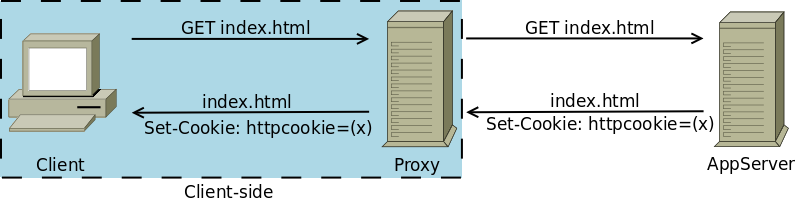
\includegraphics[width=.7\textwidth]{img/clientside-proxy-1.png}
		\label{fig:clientside-request}
	}\\
	\subfloat[An outgoing request containing a cookie set via HTTP, and one set via JavaScript. The JavaScript cookie is stripped from the request by the proxy.]{
		\label{fig:clientside-response}
		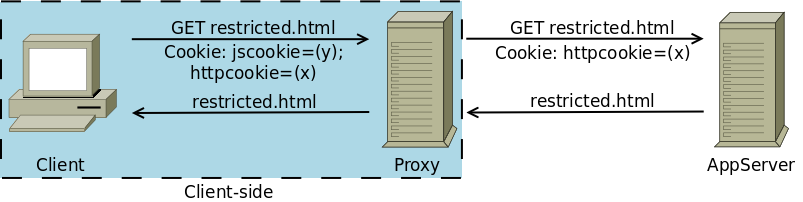
\includegraphics[width=0.7\textwidth]{img/clientside-proxy-2.png}
	}
	\caption{Client-side solution to session fixation}
	\label{fig:clientside-proxy}
\end{figure}

We want to apply the policy only to \glspl{session cookie}, instead of all cookies. To see why, consider the scenario where a user can set the theme of the current web page by clicking a button\footnote{The website \url{http://www.last.fm}, for example, allows a logged in user to set his theme by clicking the `paint it black' link at the top of the site.}. Because this theme can immediately be applied (by changing the page's css style on the fly), there is no need to send an extra HTTP request to refresh the page. To make this style change persistent, a cookie has to be set in the user's browser. To avoid the need for another HTTP request and response, this cookie is set using JavaScript. Subsequent requests will however send this cookie over HTTP, to make sure that the returned page is using the correct style. If no distinction is made between session cookies and other cookies, sending this cookie over HTTP would not be allowed by our policy. Correctly identifying which cookies are session cookies is the subject of the next section.

The proposed policy effectively mitigates the attack vectors we considered to be in scope. Cookies set from JavaScript are marked as untrusted, which mitigates the cross-site scripting attack vector, both within one domain as for sites sharing cookies across subdomains. A second attack vector is the injection of cookies through the \texttt{<meta>}-tag. Since these cookies do not come from a \texttt{Set-Cookie} header, they too are considered untrusted. As with the cross-site scripting attack vector, attacks within one domain and across subdomains are mitigated. In section \ref{evaluation}, we show that dismissing untrusted session cookies has no impact on the user experience. The complete policy is summarized in table \ref{tab:nofix-policy}.

\begin{table}[ht]
	\centering
	\begin{tabular}{r|cc}
		& Normal Cookie & Session Cookie\\
		\hline
		Trusted Channel & Allowed & Allowed\\
		Untrusted Channel & Allowed & Not Allowed\\
	\end{tabular}
	\caption{The client-side policy for preventing session fixation}
	\label{tab:nofix-policy}
\end{table}

\section{Identifying session identifiers}\label{detecting-sids}

Because there is no standardized way of doing session management (see section \ref{session-management}), we have to look for patterns which are common among session identifiers. Based on the properties of secure web sessions listed in section \ref{secure-sessions}, and on an algorithm defined by Nikiforakis et al. \cite{Nikiforakis2010}, we identify a cookie to be a session cookie if it has one of the following properties:
\begin{itemize}
	\item The name of the cookie is in a list of known session identifiers, such as \texttt{phpsessid}, \texttt{aspsessionid} and \texttt{jspsession}. Most frameworks implementing a session mechanism have default names for their session IDs, which are included in this list.
	\item The name of the cookie contains the substring `sess' and the value of the cookie is a sufficiently long string containing both numbers and characters.
	\item The cookie value passes a randomness test. For this, the relative entropy of the cookie value is computed based on the Shannon Entropy measure \cite{Kaplan2002}. Afterwards, it is calculated how many bits would be needed to encode the string \cite{Nikiforakis2010}.
\end{itemize}

\section{Implementation}

The solution was first prototyped as a lightweight HTTP proxy written in Python, and later implemented as an add-on for Mozilla Firefox\footnote{This add-on is available for download at \url{https://spideroak.com/share/IJZGC3I/pub/home/bram/Openbaar/NoFix.xpi}.}. We first discuss the advantages and disadvantages of an implementation as a browser extension. Afterwards, we discuss the relevant parts of the Firefox architecture. We conclude with the specifics about the implementation itself.

\subsection{HTTP proxy or browser extension?}

Implementing the policy as a browser extension has numerous advantages over an implementation as a HTTP proxy. The most important advantage is visible when an encrypted (\gls{https}, see section \ref{ssl}) connection is used. In this case, a browser extension is already behind the regular SSL endpoint. A HTTP proxy, however, should provide its own SSL endpoint if it wants to intercept secured traffic. This means that it should handle encryption, handshakes and certificates -- which are all very difficult to get right -- separately from the browser. The other option is to not let the proxy intercept HTTPS traffic, rendering it incapable to protect this kind of traffic against session fixation. This would be a major security compromise, since SSL traffic is deemed to be more secure than normal (unencrypted) traffic.

A second advantage lies in the fact that an extension can differentiate between the normal and private browsing modes in the browser. Thus, it can make sure normal surfing cookies are never mixed with private surfing cookies. A proxy would allow cookies that were set during a private browsing session to pass through in a normal browsing session.

An additional advantage is that a browser already has an up-to-date list of top level domain names. This is convenient when checking whether a website is trying to set a cookie for a valid parent domain (and not a top level domain).

Lastly, installing a browser extension -- and especially a Firefox add-on -- is trivial, allowing us to reach a broad audience.

There are also some disadvantages a browser extension has compared to a proxy. The most obvious one is that a particular extension implementation will only be usable by at most a few browsers, while a proxy can protect all HTTP traffic that passes through. Moreover, some browsers do not provide support for extensions at all.

Secondly, on some browsers, extensions are able to interfere with one another. This allows rogue browser extensions to thwart security extensions \cite{Barth2010}.

\subsection{The Firefox architecture}

Mozilla Firefox allows to extend the browser using a combination of JavaScript and XML. These can access the browser's XPCOM components, which offer access to various browser features.

In order to implement our client-side protection technique, the following capabilities are needed:
\begin{itemize}
	\item Inspect incoming HTTP(S) requests, to be able to track what trusted session identifiers are set.
	\item Persistently store information, to be able to keep information on persistent session identifiers.
	\item Inspect and modify outgoing HTTP(S) requests, to be able to strip out untrusted session identifiers.
\end{itemize}
These capabilities are provided by the following Firefox components:
\begin{itemize}
	\item The \texttt{http-on-examine-response} observer allows us to intercept HTTP responses before they are processed. Whenever a response is received, this object's \texttt{observe()} method is executed \cite{MozillaObservers}.
	\item The \texttt{http-on-modify-request} observer allows us to intercept and modify HTTP requests before they are sent. Whenever a response is received, this object's \texttt{observe()} method is executed \cite{MozillaObservers}.
	\item The \texttt{storageService} allows us to persistently store data in a SQLite database \cite{MozillaStorage}. This service is also used by Firefox internally to store data on the local machine \cite{Bonne2011}.
\end{itemize}

Additionally, Firefox provides an interface that examines a hostname and determines the longest portion that should be treated as though it were a top-level domain (\gls{tld}) \cite{MozillaDevelopers2010}. This is convenient when checking whether a cookie is being set for an allowed domain.

It must be noted that the previously listed `required capabilities' are currently only partially available in all other browsers. Google Chrome, for example, had no support for intercepting HTTP requests and responses at the time of writing, although this feature is currently on their wishlist \cite{ChromiumWishlist}. To be able to port the add-on to other browsers, these browsers should implement similar interfaces.

\subsection{Implementation as a Firefox add-on}

The proposed policy was implemented as a Firefox add-on, available for Firefox 3.5 or higher. We describe the internals of the add-on in this section.

To detect when a trusted session ID is set, the add-on searches for a \texttt{Set-Cookie} header in all incoming HTTP responses. When it finds that a cookie is being set, it checks whether the cookie is a session identifier, using the algorithm described in section \ref{detecting-sids}. If the cookie contains a \texttt{domain} attribute, the value of this attribute is checked for validity in order to prevent cross-site cooking attacks \cite{Zalewski2006} against the add-on. For this, the add-on assures that \texttt{domain} parameters in cookies are always parent domains or subdomains of the website the cookie was received from. Also, Firefox' top-level domain list \cite{MozillaDevelopers2010} is used to make sure no website can set a cookie for a top-level domain (such as \emph{.co.uk}).

When all requirements are satisfied, the cookie is stored in a separate cookie jar implemented as a SQLite database. Storage handled using asynchronous writes, to reduce the delays introduced by the add-on (see section \ref{performance}). To make sure that session IDs are also available before their write operation is complete, cookies are temporarily stored in main memory until they have been written to the database.

To filter untrusted session IDs, every outgoing HTTP request is intercepted by the add-on. Before a request is sent to the server, its \texttt{Cookie} header is inspected. For each cookie, the add-on checks whether the cookie represents a session identifier. If this is the case, the add-on's separate cookie jar is queried to make sure that the cookie is trusted. If this is not the case, this particular cookie is stripped from the request. After having repeated this process for all cookies, the request is released with the modified \texttt{Cookie} header.

\section{Evaluation}\label{evaluation}

The add-on was evaluated in three parts. The first part evaluates the add-on's functional correctness. The second part evaluates its impact in real-world browsing scenarios. Lastly, the third part evaluates the add-on's performance, and thus -- together with the second part -- its impact on everyday web browsing.

\subsection{Correctness}

To make sure that the implementation behaves in accordance with the specification, a simple HTTP server was created. This server issues both cookies in the way a session fixation attack would, as in the way a legitimate website would. It is then checked that only the trusted session identifiers are returned to the server on subsequent requests, while untrusted session identifiers are stripped. The implementation passed all these correctness tests.

\subsection{Real-world impact}

An evaluation of the add-on's impact on the user experience is difficult to automate. Because of this, we asked several test persons to use the add-on during their daily web browsing activities. Apart from collecting logging data from the test persons, we asked them to pay close attention to see if any websites would break or behave differently. The experiment ran for 20 weeks.

From the log files, we found that in a considerable fraction (19.53\%) of the requests, session cookies were stripped. We would assume that, with such statistics, the extension leads to a severely degraded user experience. Surprisingly, the only problems that were mentioned by the testers had other causes such as malfunctioning websites or other poorly written add-ons. Not a single problem mentioned in these 20 weeks was due to the policy applied by our add-on. We will discuss the causes for this behavior in section \ref{discussion}.

Because of the very little real-world impact of this solution, it would even make sense for Firefox to implement the described policy by default. In the past, the Firefox team has already taken bold steps to increase security, even though some websites might have been broken afterwards. \cite{Singh2010,MozillaXmlHttp,Bonne2011}

\subsection{Performance}\label{performance}

The user experience can also be negatively impacted by a large overhead induced by client-side protection mechanisms \cite{Bonne2011}. We quantify this performance overhead by performing two experiments.

The first experiment consisted of timing the delays that were introduced by the add-on during an everyday web browsing session. For this, timers were added to the add-on code. We measured that the average delays for requests (where it is checked whether a cookie is allowed) and responses (where cookies are set) were 1.25\ ms and 0.25\ ms, respectively.

The second experiment\footnote{This experiment was performed by Nick Nikiforakis \cite{Bonne2011}.} that was performed compares the \emph{page} load times in Firefox with and without the add-on enabled for the top 1000 most visited pages on the internet, according to Alexa \cite{Alexa1000}. For this experiment, we used a setup similar to the one used to evaluate SessionShield \cite{Nikiforakis2010}, where the network inconsistencies are eliminated by hosting all the pages locally. A fake local DNS server and fake local web server are used to serve the captured pages. For additional resources (e.g. images, scripts), the local web server responds with a 404 `page not found' status code. The actual experiment consists of using the ChickenFoot add-on \cite{ChickenFoot} to automate the process of starting a timer, instructing Firefox to load a page, and stopping the timer. This scenario is repeated three times for every web page, both with and without the add-on enabled. The average page-load time without session fixation protection is 195.407\ ms. When our add-on is enabled, the average page-load time is 198.242\ ms \cite{Bonne2011}. Thus, the average overhead introduced by our add-on is approximately 3\ milliseconds, which is negligible compared to the more than 0.5\ seconds average loading time for pages on the internet \cite{Webmetrics}.

\section{Discussion}\label{discussion}

Our client-side countermeasure against session fixation is very effective with no impact on the user experience and a minimal impact on the site's behavior in the form of false positives \cite{Bonne2011}. In this section, we describe why the add-on blocks so many cookies, and why this does not affect the web application's behavior or the user experience.

One reason is that a web application might not need cookies that are set via JavaScript to be available in HTTP requests. Indeed, when a cookie is set via JavaScript, chances are quite high that this cookie will afterwards only be accessed via JavaScript.  However, a JavaScript cookie will also always be sent over HTTP, and thus stripped by the add-on. The reason that this does not impede a web application's behavior is that when the web application tries to access such a cookie using JavaScript, it is allowed to do so by our policy. Thus, a web application accessing untrusted cookies via JavaScript only will keep working as expected.

Another reason for the stripped cookies is that the add-on also exhibits some false positives \cite{Bonne2011}. False positives are cookies that should be allowed to be sent over HTTP, but which were erroneously stripped from the request. The cookies that we discovered to be false positives when implementing and evaluating the add-on were all related to web analytics services. Web analytics services provide a way for web developers to gather statistics about their website. Two examples of web analytics services are Google Analytics\footnote{An overview of the features available in Google Analytics can be found on \url{http://www.google.com/analytics/features.html}.} and Yahoo! Web Analytics\footnote{An overview of the features available in Yahoo! Web Analytics can be found on \url{http://web.analytics.yahoo.com/features}.}. To be able to track a visitor's behavior on a website, these services set cookies to measure the time spent on the website, and to uniquely identify a visitor \cite{Tappenden2009,GoogleAnalytics}. This last category of cookies often has a value that is random, and because the web analytics code is embedded as JavaScript code within the developer's web page, this type of cookie is set via JavaScript. Hence, these cookies will be marked as `untrusted' by the add-on, and will as such be stripped from all HTTP requests. Stripping these cookies only affects the web developer, which is why none of the add-on testers noticed a degraded user experience.

If we want our policy to be widely adopted, we should make sure that the previously mentioned false positives are accounted for, even if they don't impede the user experience. Because of this, we also provide a whitelist of cookies that should not be stripped in the add-on.

\section{Extending with session hijacking protection}

The add-on was also extended with a solution to the session hijacking attack. To do this, we made an even stronger distinction between HTTP cookies and JavaScript cookies: in our extended policy, session cookies that are set via HTTP are not allowed to be accessed by JavaScript. This prevents session cookies from being stolen via \gls{xss} attacks.

The policy extension is implemented in our add-on by adding the \texttt{HttpOnly} flag to every incoming HTTP cookie which is marked as a session cookie. When this flag is enabled, the browser will only allow the cookie to be read via HTTP (see section \ref{httponly} for more information). Thus, we let the browser handle the blocking of HTTP session cookies over JavaScript. Figure \ref{fig:clientside-httponly} shows the adapted version of Figure \ref{fig:clientside-request}, with the solution extended to provide session hijacking protection.

\begin{figure}[ht]
	\centering
	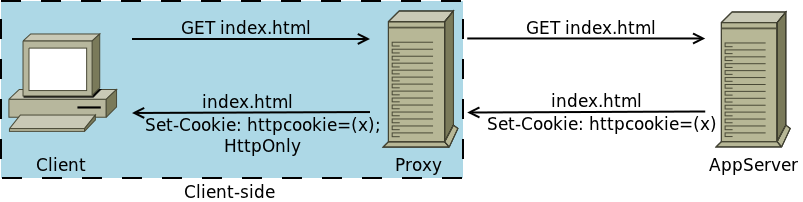
\includegraphics[width=.7\textwidth]{img/clientside-proxy-3.png}
	\caption{Client-side solution to session fixation and session hijacking}
	\label{fig:clientside-httponly}
\end{figure}

The extension to our policy is related to the session hijacking solution proposed by Nikiforakis et al. \cite{Nikiforakis2010} (which was be discussed in section \ref{sessionshield}), where HTTP cookies are kept in a separate cookie store, outside of the browser. The difference lies in the fact that our add-on \emph{does} allow the browser access to the cookies. The only access our extended policy prevents is from JavaScript to session cookies.

\section{Comparison with other session attack countermeasures}\label{related-work}%TODO

In this section, we compare our solution to some of the countermeasures which were described in the previous chapter. At the end of this section, we give an overview of the countermeasures, and which scenarios they protect against. %TODO

\subsection{HttpOnly}\label{httponlyremark}

HttpOnly cookies, as described in section \ref{httponly}, are cookies that are only accessible by HTTP. A web developer may think that setting the \texttt{HttpOnly} flag for every session cookie would prevent an attacker from using XSS to inject another value for these cookies. However, when the attacker sets the cookie before the web server does, \emph{he} is the one who can decide whether the \texttt{HttpOnly} flag is set. Thus, the web developer would have to make sure that a cookie is always set before an attacker can set it.

Moreover, even if the web server is able to set the session cookie before the attacker does, the attacker is often still able to set a cookie with the same name as the session cookie for the parent domain, as we described in section \ref{subdomain-setting}. This causes the browser to send both the parent domain cookie and the subdomain cookie when a page on the subdomain is accessed. Since the \texttt{domain} attribute isn't attached to cookies in the request, the server has no way of distinguishing between both cookies. Thus, although it is recommended to set the \texttt{HttpFlag} on cookies whenever possible, this will not completely solve the session fixation attack.

\subsection{One-time cookies}

% Het belang van scheiden van authenticatie cookies en andere cookies
% Om deze reden OTC niet beschikbaar via JS.
% Moet aan server kant geïmplementeerd worden

\subsubsection{Session fixation solution by Johns et al.}

% Stellen voor om proxy ook aan client-side toe te passen in paper, gaat niet zie onze paper
% Configureren van elke server is niet haalbaar voor client-side solution, dus: heuristieken

\subsection{SessionShield}
% Kritisch: hoe lost dit javascript cookies op?

\chapter{Conclusion}


\backmatter
\bibliography{/home/bram/Documenten/library,/home/bram/Documenten/rfc,/home/bram/Documenten/extra}\bibliographystyle{plainurl}

\end{document}


